\appchapter[Reinforcement Learning Agent Evaluation]{Reinforcement Learning Agent Evaluation}
\label{appendix:e}

\begin{figure}[ht]
  \centering
  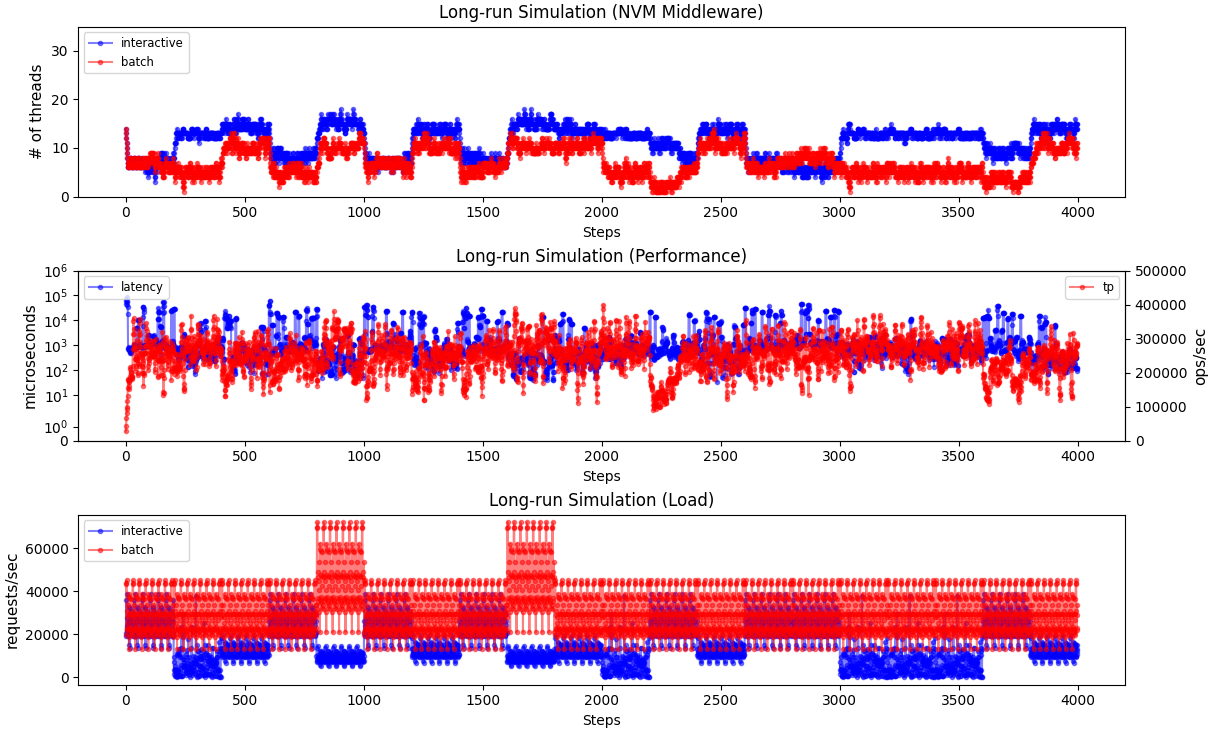
\includegraphics[width=\textwidth,height=\textheight,keepaspectratio]{images/long_run_sim.png}
  \caption[Reinforcement Learning Agent Adaptation to Shifting Workloads]{Illustration demonstrating the dynamic adjustment of thread counts by the RL agent during a test comprising 4,000 steps with randomly alternating phases. The top row showcases the RL agent's utilization of learned knowledge to optimize the number of interactive and batch threads for each phase. In the middle row, the throughput and 99th percentile latency reported by the NVM Middleware at each time step are depicted. By dynamically modifying the NVM Middleware threads, the throughput aligns with the predefined throughput SLA. However, unexpected spikes in the 99th percentile latency are observed, contrary to the training phase. The bottom row illustrates the operations per second sent by each phase, highlighting the shift in patterns every 200 steps.}
  \label{fig:long_run_eval}
\end{figure}

\begin{table}[ht]
    \centering
    \caption[Reinforcement Learning Agent Reward Analysis in Long-run Test]{Analysis of the rewards achieved by the RL agent under shifting workloads compared to two baseline scenarios: one without concurrency control and the other keeping the NVM Middleware threads fixed. The values represent the distribution of reward signals reported by the environment at each time step, ranging from the minimum to the maximum observed, along with quartiles and median scores. Overall, the NVM Middleware with the RL agent achieves the highest reward.}
    \label{table:eval_results_reward}
    % Tabular environment goes AFTER the caption!
    % \begin{adjustbox}{width=1\textwidth}
    \begin{tabular}{|c|c|c|c|}
      % after \\: \hline or \cline{col1-col2} \cline{col3-col4} ...
      \hline
      \thead{} & \thead{No NVM Middleware} & \thead{NVM Middleware Fixed} & \thead{NVM Middleware + RL} \\
      \hline
      Min & -94755.386 & -65157.089 & -87907.434 \\\hline
      Q1 & -10790.1 & -8605.4625 & -3647.9454 \\\hline
      Median & -6983.235 & -3208.995 & -4.005294 \\\hline
      Q3 & -4042.9125 & -2.353015 & 0.31523 \\\hline
      Max & 3.174046 & 4.89667 & 4.582787 \\
      \hline
    \end{tabular}
  % \end{adjustbox}
\end{table}

\begin{table}[ht]
    \centering
    \caption[Reinforcement Learning Agent Throughput Analysis in Long-run Test]{Analysis of the throughput achieved by the RL agent under shifting workloads compared to two baseline scenarios: one without concurrency control and the other keeping the NVM Middleware threads fixed. The values represent the distribution of throughput measurements reported by the NVM Middleware at each time step, ranging from the minimum to the maximum observed, along with quartiles and median scores. Overall, the NVM Middleware with the RL agent achieves the highest throughput.}
    \label{table:eval_results_tp}
    % Tabular environment goes AFTER the caption!
    % \begin{adjustbox}{width=1\textwidth}
    \begin{tabular}{|c|c|c|c|}
      % after \\: \hline or \cline{col1-col2} \cline{col3-col4} ...
      \hline
      \thead{} & \thead{No NVM Middleware} & \thead{NVM Middleware Fixed} & \thead{NVM Middleware + RL} \\
      \hline
      Min & 72,218.9 & 104,719.9 & 159,168.8 \\\hline
      Q1 & 112,440 & 148,792.5 & 218,816.25 \\\hline
      Median & 135,508.5 & 186,877 & 252,078.5 \\\hline
      Q3 & 166,340.25 & 231,597.75 & 278,205 \\\hline
      Max & 242,104.4 & 357,445.6 & 352,800.27 \\
      \hline
    \end{tabular}
  % \end{adjustbox}
\end{table}

\begin{table}[ht]
    \centering
    \caption[Reinforcement Learning Agent Latency Analysis in Long-run Test]{Analysis of the throughput achieved by the RL agent under shifting workloads compared to two baseline scenarios: one without concurrency control and the other keeping the NVM Middleware threads fixed. The values represent the distribution of latency measurements reported by the NVM Middleware at each time step, ranging from the minimum to the maximum observed, along with quartiles and median scores. Surprisingly, in this particular test, both configurations involving the NVM Middleware exhibited higher latency compared to the baseline without concurrency control. This unexpected outcome suggests that the interactive workloads may not have adequately stressed the system, resulting in increased latency when utilizing the NVM Middleware. Further investigation is warranted to ascertain the underlying factors contributing to this behavior.}
    \label{table:eval_results_latency}
    % Tabular environment goes AFTER the caption!
    % \begin{adjustbox}{width=1\textwidth}
    \begin{tabular}{|c|c|c|c|}
      % after \\: \hline or \cline{col1-col2} \cline{col3-col4} ...
      \hline
      \thead{} & \thead{No NVM Middleware} & \thead{NVM Middleware Fixed} & \thead{NVM Middleware + RL} \\
      \hline
      Min & 19 & 89 & 130.95 \\\hline
      Q1 & 81 & 239 & 396.75 \\\hline
      Median & 19 & 674.5 & 754 \\\hline
      Q3 & 271.5 & 1888.75 & 1427 \\\hline
      Max & 82824 & 34090.93 & 34712.04 \\
      \hline
    \end{tabular}
  % \end{adjustbox}
\end{table}